%---------------------------------------------------------------
\chapter{Background}
%---------------------------------------------------------------

\begin{chapterabstract}
	\todoadd
\end{chapterabstract}

%---------------------------------------------------------------
\section{The R Language}
%---------------------------------------------------------------

\textit{R}\cite{r} is a programming language used for statistical computation and data visualization. It was developed Ross Ihaka and Robert Gentleman at the University of Auckland as an alternative to the S language. It is part of the GNU Project, licensed as a free software under GNU GPL.

The beauty of R is that very complex operations can be expressed in very few lines of code, as demonstrated in listin \ref{lst:motivation}. It is used a lot by statistician, where a big part of them are non-programmers, and this is reflected in the design of the language. It allows for high levels of abstractions, expressive domain-specific languages and APIs and code that is very

\begin{figure}[hb]
		\centering
		\begin{minipage}{0.45\textwidth}
			\centering
			\begin{minted}{R}
ggplot(
  data = gapminder,
  aes(
    x = gdpPercap, y = lifeExp,
    color = continent
  )
) +
  geom_point() +
  scale_x_log10()
      \end{minted}
      \captionof{listing}{R example\todocite}\label{lst:motivation}
		\end{minipage}%
		\hfill
		\begin{minipage}{0.45\textwidth}
			\centering
			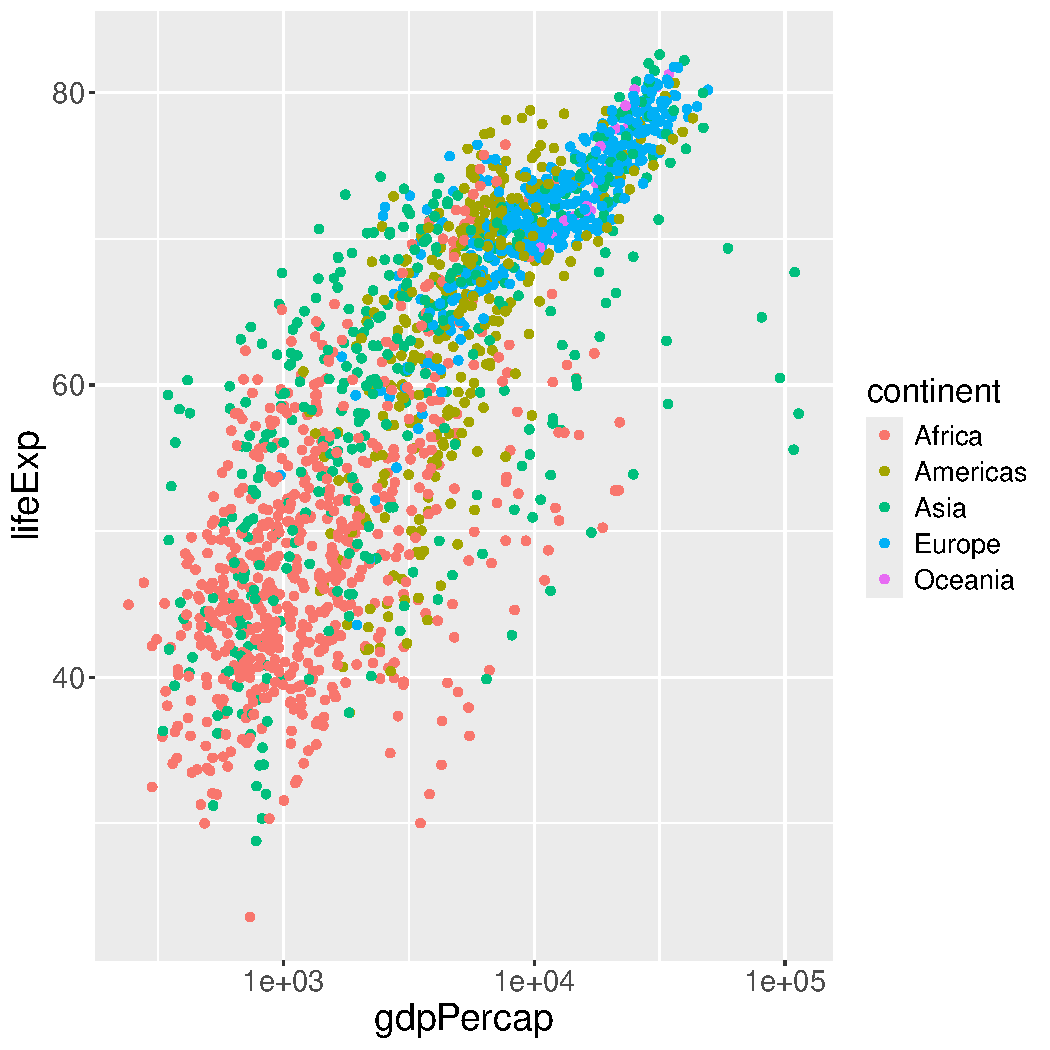
\includegraphics[width=\textwidth]{figures/motivation-Rplots.pdf}
			\caption{Plot of listing \ref{lst:motivation}}
		\end{minipage}
\end{figure}

The language is high-level, dynamic, object-oriented, functional, interpreted, and lazy, with automatic memory management.

The R syntax is very C-like, with \texttt{if} statements, \texttt{for} and \texttt{while} loops, array indexing and function calls. For assignment, the \texttt{<-} operator is used. Statements are separated by newline, optionally by semicolon if they are on the same line.

%---------------------------------------------------------------
\subsubsection*{Types}
%---------------------------------------------------------------

R basic types are the \textit{numeric types} (\textit{integer}, \textit{double} or also \textit{real} and \textit{complex}), \textit{character type} (strings) and \textit{logical type} (the boolean values \texttt{TRUE} and \texttt{FALSE}). R also has \texttt{NULL}, and a constant \texttt{NA} (\textit{not available}) representing a missing value.

R has no concept of scalars. Instead, all basic types are represented as \textit{vectors}. To create a vector with multiple elements, the function \texttt{c} (standing for combine) can be used. All the traditional mathematical operators are also vectorized.

For storing elements of different types, a \textit{list} is used. Other commonly used types built on top of vectors and lists are \textit{matrix} (two-dimensional vector), \textit{array} (multi-dimensional vector) and \textit{data frame} (matrix-like structure whose columns can have different types).

Every type can have associated \textit{attributes}, a collection of name-value pairs. These are accessed via the \texttt{attr} or \texttt{attributes} functions.

R also has multiple \textit{object models}. The most common ones are \textit{S3}, which is controlled by setting a \texttt{class} attribute on any type, and \textit{S4}, which defines more formal classes which have to be created and instantiated, and are internally represnted by a distinct type.

%---------------------------------------------------------------
\subsubsection*{Environments}
%---------------------------------------------------------------

Different scopes in R are separated using objects named \textit{environments}. An environment consists of a \textit{frame}, which is the collection of variables, and a pointer to an \textit{enclosing environment} (also called a \textit{parent}). The topmost environment has a pointer to a special \textit{empty environment}, which has no other parent.

When a variable or a function is accessed, it is first looked for in the current environment. If not found, it is searched for recursively in each enclosing environment. Only then if it is not found, it is an error.

The lookup for functions is separate from non-function lookup. An assignment of a variable in some environment does not shadow a function in its enclosing environment. So the code \texttt{c <- 42; c(c, c)} results in one vector with two numbers 42, because the definition of the variable \texttt{c} does not shadow the function of the same name from the base environment.

These environments are also first-class values. We can create new environments, access the value of the currently executed one , or even access and modify environments on the call stack.

%---------------------------------------------------------------
\subsubsection*{Functions}
%---------------------------------------------------------------

A \textit{function}, or also a \textit{closure}, is composed of three parts - \textit{formals}, which is the list of formal arguments and their default values, \textit{body}, which is the code of the function, and \textit{environment} defining the lexical scope of the function body. New functions can be created with the \texttt{function} keyword.

Most operations that happen in R are in fact function calls. This includes the control flow statements (like \textit{if} or \textit{while}), binary operations, assignment, and even surrounding an expression with parenthesis or multiple expression with braces. This is demonstrated in listing \ref{lst:r-special-calls}. Note that built-in functions have to be surrounded with backticks in order to referr to them as identifiers.

\begin{listing}[ht!]
	\begin{sublisting}[t!]{0.47\textwidth}
		\centering
		\begin{minted}{R}
a <- if (TRUE) {
  1
} else
  2 * (3 + 4)
    \end{minted}
	\end{sublisting}
	\hfill
	\begin{sublisting}[t!]{0.47\textwidth}
		\centering
		\begin{minted}{R}
# This is equivalent to
# the previous statement
`<-`(a, `if`(
  TRUE,
  `{`(1),
  `*`(
    2,
    `(`(`+`(3, 4))
  )
))
    \end{minted}
	\end{sublisting}
	\caption{Demonstration of R special calls}\label{lst:r-special-calls}
\end{listing}

%---------------------------------------------------------------
\subsubsection*{Laziness}
%---------------------------------------------------------------

R is lazy in arguments. This means that when a function is called, the passed arguments are not instantly evaluated, but are instead wrapped in a \textit{promise}, a tuple of \textit{expression}, \textit{value}, and \textit{environment}. The value is at first set to the unbound value. When the promise is first accessed, the expression of the promise is evaluated with its environment (also called a \textit{force}). The result is cached in the value field, and every other access to the argument results in the cached value.

This can be seen in example \ref{lst:example-lazy}. The call at line 12 first prints \enquote{Hello from g}, then the parameter \texttt{x} is accessed, the promise is forced, and the text \enquote{Hello from f} is printed. The second call to the function \texttt{h} demonstrates a second behavior - when a parameter is never accessed, the promise is not evaluated, and nothing is printed.

\begin{listing}[h!]
	\centering
	\begin{minted}{R}
f <- function(x) {
    print("Hello from f")
    x
}

g <- function(x) {
    print("Hello from g")
    x
}

# Prints "Hello from g", then "Hello from f"
g(f(42))

h <- function(x) 0

# Does not print anything
h(f(42))
  \end{minted}
	\caption{Example of R laziness}\label{lst:example-lazy}
\end{listing}

Being lazy in the arguments allows R to have very expressive domain-specific languages for ease of manipulating the data, as well as reducing memory overhead of the programs.

Promises can also be created manually by calling the \texttt{delayedAssign} function or from the C API.

%---------------------------------------------------------------
\subsubsection*{Immutability}
%---------------------------------------------------------------

All R values are \textit{semantically immutable}, with the exception of environments. This means that when a variable holds a value, this value never changes unless the variable is reassigned. We say that non-environment values have a \textit{copy-on-write behavior} - when a value is modified, a new copy is created with the modified parts.

Thanks to the syntax of R, it is possible to write code that looks like it is using mutability, but keeps the copy-on-write behavior. In the example \ref{lst:imm}, the statement on line 3 looks like it is mutating the vector in place, but instead the function \texttt{[<-} is called, which creates a copy of the vector, modifies it and reassigns the variable x.

The only truly mutable values are environments, and they conform to a \textit{reference behavior}. Listing \ref{lst:envir} shows this behavior - the variable \texttt{x} is added to both \texttt{e1} and \texttt{e1}, even though we only defined it on \texttt{e2}.

\begin{listing}
	\centering
	\begin{minipage}{0.47\textwidth}
		\begin{minted}{R}
x <- c(1, 2, 3)
y <- x
y[1] <- 42
# x is still vector (1, 2, 3)
      \end{minted}
		\caption{Immutability example}\label{lst:imm}
	\end{minipage}
	\hfill
	\begin{minipage}{0.47\textwidth}
		\begin{minted}{R}
e1 <- new.env()
e2 <- e1
e2$x <- 42
e1$x == 42
# TRUE
      \end{minted}
		\caption{Example of environment mutability}\label{lst:envir}
	\end{minipage}
\end{listing}

%---------------------------------------------------------------
\subsubsection*{Reflection}
%---------------------------------------------------------------

As mentioned before, environments are a first-class citizen. This allows for any function to access and even modify any environment where it was created or called. Moreover, when combined with lazy arguments, a function can reflect on the environment it is being forced in and modify it, sometimes in unpredictable ways.

This is demonstrated in listing \ref{lst:bad-ref}, where we call to \texttt{good}, inside of which we evaluate to the call to \texttt{bad}, which reflects on the caller environment, deletes a binding, and results in a unbinded variable on line 9.\todo{rewrite}

\begin{listing}
	\centering
	\begin{minted}{R}
bad <- function() {
  rm("x", envir=sys.frame(-1)) # Remove the variable x from the caller
  2
}

good <- function(y) {
  x <- 1
  z <- y # Here the promise is evalated
  x + z
}

good(bad())
# Error in good(bad()) : object 'x' not found
  \end{minted}
	\caption{Example of malicious reflection\todocite}\label{lst:bad-ref}
\end{listing}

R also has primitives for creating, manipulating, and evaluating expressions from the language itself. This allows for, among other things, evaluate a promise under a different environment, programatically create arbitrary pieces of code, or instrument functions with additional calls \todo{different example \dots}.

Combining reflection, laziness and side effects makes R a very complex language to optimize.

\newpage
%---------------------------------------------------------------
\section{GNU-R}
%---------------------------------------------------------------

The R language is not formally specified, it only has a reference implementation that we will refer to as \textit{GNU-R}. It is written in the C programming language and spans over more than {250 000} lines of code.

%---------------------------------------------------------------
\subsubsection*{Representation}
%---------------------------------------------------------------

The GNU-R represents all code and values as \textit{symbolic expressions} (also \textit{S-expressions} or \textit{sexps}), a format for nested lists, popularized by the Lisp languages. The type \texttt{SEXP} is a pointer to either a \texttt{SEXPREC} or \texttt{VECTOR\_SEXPREC} structure. Both of these structures contain a header of type \texttt{sxpinfo\_struct}, a pointer to the attributes of the current value, and previous and next nodes in the garbage collector. The header then contains \texttt{SEXPTYPE}, the type of the \texttt{SEXP} (values are defined as in \ref{tbl:sexptype}), as well as additional attributes with information about the type, garbage collection and debug information. The rest of the structure cointains the actual data. The structure of a \texttt{SEXP} value is represented in figure \ref{fig:sexp-struct}.

\begin{figure}
	\centering
	\begin{adjustbox}{trim=5pt 20pt 0 40pt, clip}
		\includediagram{0}
	\end{adjustbox}
	\caption{Structure of the GNU-R \texttt{SEXP} type}\label{fig:sexp-struct}
\end{figure}

\begin{table}[h!]
	\begin{tabular}{c l l}
		\textbf{no} & \textbf{SEXPTYPE} & \textbf{Description}       \\
		\hline
		0           & NILSXP            & NULL                       \\
		1           & SYMSXP            & symbols                    \\
		2           & LISTSXP           & pairlists                  \\
		3           & CLOSXP            & closures                   \\
		4           & ENVSXP            & environments               \\
		5           & PROMSXP           & promises                   \\
		6           & LANGSXP           & language objects           \\
		7           & SPECIALSXP        & special functions          \\
		8           & BUILTINSXP        & builtin functions          \\
		9           & CHARSXP           & internal character strings \\
		10          & LGLSXP            & logical vectors            \\
		13          & INTSXP            & integer vectors            \\
		14          & REALSXP           & numeric vectors            \\
		15          & CPLXSXP           & complex vectors            \\
		16          & STRSXP            & character vectors          \\
		17          & DOTSXP            & dot-dot-dot object         \\
		18          & ANYSXP            & make “any” args work       \\
		19          & VECSXP            & list (generic vector)      \\
		20          & EXPRSXP           & expression vector          \\
		21          & BCODESXP          & byte code                  \\
		22          & EXTPTRSXP         & external pointer           \\
		23          & WEAKREFSXP        & weak reference             \\
		24          & RAWSXP            & raw vector                 \\
		25          & OBJSXP            & objects not of simple type \\
	\end{tabular}
	\caption{The different SEXP types\cite[1.1.1 SEXPTYPEs]{rprojectInternals}}\label{tbl:sexptype}
\end{table}

These structures are not available directly, the \texttt{SEXP} is exported as an opaque pointer type. Individual fields are accessible via exported functions.

%---------------------------------------------------------------
\subsubsection*{Interpreter}
%---------------------------------------------------------------

The GNU-R parses the code to an \textit{abstract syntaxt tree} (\textit{AST}), also represented with \texttt{SEXP}s with the \texttt{LANGSXP} type.

After the first execution of a function or by calling \texttt{compiler::cmpfun} on it, the function is passed to a \textit{bytecode compiler}, written in R. The bytecode is stack-based with fat instructions, like specialized instructions for \texttt{for} loops, or \todo{\dots}. The

When a function is compiled, its \texttt{SEXP} is modified in-place, replacing the AST body with a bytecode. Every other call to this function is then interpreted by the bytecode interpreter, which is written in C and is also is part of the GNU-R.

An example of the bytecode can be seen in \texttt{todo}.

\todo{interpreter optimizes (if, +, assume plus in plus, constfold)}

%---------------------------------------------------------------
\subsubsection*{Garbage Collector}
%---------------------------------------------------------------
R does not have primitives for managing memory, instead an automatic memory management provided by the runtime is expected. GNU-R uses a generational non-moving stop-the-world garbage collector with three generations\cite{r-gc-notes}.

Next to the GC, GNU-R also has a reference counter for each object, included in the object header. This is used for optimistic mutations - when an object would be copied and mutated, but there is only one reference to it, it is instead mutated in place, avoiding an unnecesarry copy. This correctly preserves the copy-on-write behavior.

%---------------------------------------------------------------
\subsubsection*{C API}
%---------------------------------------------------------------

In order to speed-up certain packages and libraries, GNU-R allows parts of the code to be written in more low-level languages, accessed via a C API. This includes the definitions for the SEXP type, a big set of functions and macros to manipulate these types, as well as

This feature is more of an after thought more than a deliberate choice, as indicated for example by the the main file with the type definitions being called \texttt{Rinternals}. Big portion of the internal implementation is exposed as part of the API and even parts that are supposted to be hidden are sometimes used by the package authors. For example, even though the SEXP type is exported as an opaque pointer, some packages are still accessing the underlying structures in order to manipulate them.

This makes evolution of GNU-R without breaking packages very hard, as well as complicating alternative implementations of R, as they need to explicitly export the same functions as GNU-R if they want to support all available libraries.

\newpage
%---------------------------------------------------------------
\section{The Ř compiler}
%---------------------------------------------------------------

\textit{Ř} (also stylized as \textit{Rsh}) is a just-in-time compiler for the R language, developed at Programming Languages Laboratory at Czech Technical University in Prague\footnote{\url{https://prl-prg.github.io/}} and Programming Research Laboratory at Notheastern University\footnote{\url{https://prl.khoury.northeastern.edu/}}. The project is freely available and hosted on GitHub.

It is built as an extension to GNU-R, although it uses a slightly modified version of the codebase. It bypasses the GNU-R bytecode compiler and interpreter, instead using a custom one, while reusing the \texttt{SEXP} representation, AST interpreter, and garbage collector.

For the compilation to native code, the \textit{LLVM Project}\cite{llvm} is used.

The compilation pipeline is outlined in figure \ref{fig:rsh-archit}

\begin{figure}
	\centering
	\includediagram[0.7]{3}
	\caption{Overview of Ř architecture\cite{reusing-jit}}\label{fig:rsh-archit}
\end{figure}

%---------------------------------------------------------------
\subsubsection*{Runtime objects}
%---------------------------------------------------------------

Ř uses the GNU-R \texttt{SEXP} representation and memory management. All runtime objects are embedded into the SEXP objects. This is one of the modifications that need to be applied to GNU-R, a new \texttt{SEXPTYPE} is added (\texttt{EXTERNALSXP}), along with the necessary changes to how it is collected and how it references other objects.

The structure of Ř runtime object can be seen in figure \ref{fig:rsh-object-struct}. It represented as the \texttt{SEXP} header, the \texttt{SEXPTYPE} alwyas set to the \texttt{EXTERNALSXP}, and then the embeded \texttt{RirRuntimeObject}. This object always starts with two \texttt{uint32\_t} numbers, the first dictates how many bytes after the start of the Ř object do start the pointers to the other \texttt{SEXP}s, and the second indicates how many pointers are there. The magic number dictates which Ř object it is.

There are helpers macros to access the headers, as well as the pointers to other \texttt{SEXP}s. On the Ř side, there are functions to convert between a C++ pointer and a SEXP.

\begin{figure}
	\centering
	\begin{adjustbox}{trim=10 80pt 0 0, clip}
		\includediagram{1}
	\end{adjustbox}
	\caption{Structure of the Ř runtime objects}\label{fig:rsh-object-struct}
\end{figure}

The composition of Ř objects can be seen in figure \ref{fig:rsh-composition}.

The centerpiece of a Ř function is a \textit{dispatch table}. This represents a single function with multiple compiled version, each having an individual entry in the dispatch table. The first version is also called a \textit{baseline}, and it is the bytecode interpreted version without any speculations.

Every function is then represented by a \texttt{Function} structure. This holds the signature of the function, the context for contextual dispatch (see \todo{chapter}), statistic about the execution like how many times it has been invoked or deopted, the body of the function and the type feedback.

The body of a function is stored in a structure called \texttt{Code}. This is either a bytecode body or a pointer to the native function, and the constants pool.

The \textit{feedback} collected from a bytecode interpretation consists of three different types of observations in a structure \texttt{TypeFeedback}. \textit{Observed calls} records the destination of  a called function. \textit{Observed types} record the types of values that are loaded from environment, forced, or are results of a function call. \textit{Observed tests} has four values recording how a branch was taken (\texttt{None}, \texttt{OnlyFalse}, \texttt{OnlyTrue} and \texttt{Both}). Since every function has different number of slots for each observation slot, the \texttt{TypeFeedback} object has different size for each function. \todo{flexible array member}

\begin{figure}
	\centering
	\includediagram[0.7]{2}
	\caption{Composition of Ř runtime objects}\label{fig:rsh-composition}
\end{figure}

% \rirexample

%---------------------------------------------------------------
\subsubsection*{RIR bytecode interpreter}
%---------------------------------------------------------------

The bytecode used by Ř is called \textit{RIR}. It is a stack-based bytecode, interpreted by a Ř interpreter. It uses the GNU-R bytecode execution stack. Unlike the GNU-R bytecode, the RIR instructions are much more granular, there are fewer of them, they are not as specialized and a single instruction represent much smaller piece of C code that in GNU-R. The RIR is also much less optimized, due to being only an interpreter intended to be further optimized, whereas the GNU-R bytecode is the final compilation stage.

Similarly to the GNU-R compiler, when a function is compiled to \texttt{RIR}, its body gets replaced with a \textit{dispatch table}.

\todo{how is a loop hijacked}

For this thesis, the important bytecode instructions are \texttt{record\_call\_}, \texttt{record\_type\_}, and \texttt{record\_test\_}. These do the recording of feedback information about calls, types and tests respectively. The semantics of the instructions is observing the top value on the stack and record the information to the \texttt{TypeFeedback} structure on an index stored as an immediate. As a note, when disassebling RIR, these instructions are not printed, instead the slot they are recording to is, along with the label as \texttt{Call\#N}, \texttt{Type\#N} or \texttt{Test\#N}.

Apart from the runtime values, the RIR interpreter also records other informations about the running program, most notably the number of times a function has been invoked, and the number of times a loop has been executed. These are used to determine which parts of the program are executed frequently, and thus are a good candidates for compiling to native code.

%---------------------------------------------------------------
\subsubsection*{PIR compiler}
%---------------------------------------------------------------
When a function or a loop is determined to be hot, it is compiled to \textit{PIR}, an intermediate representation used for the compilation to native code.

PIR is composed of instruciton in a \textit{static single-assignment form} (\textit{SSA}), organized in \textit{basic blocks}, with each block being terminated with a (conditional) jump to another basic block, or a speculation checkpoint.

Every instruction has a type (also called a \textit{PIR type}), which model the R types as well as additional information. It also contains an explicit list of effects, which include visibilty (a state of global flag determining if a result is written to stdout), warn and error (\todo{\dots}), force (it might force a promise), deopt (instruction can trigger a deoptimization), or

\todo{example instruction}

\todo{speculative optimizations}

After all of the optimizations are finished, the PIR code is transformed into \textit{LLVM bitcode}, the intermediate representation of LLVM. This is then passed to the \textit{ORC JIT compiler}, which is part of the LLVM project and which does the lowering itself.

%---------------------------------------------------------------
\subsubsection*{Contextual dispatch}
%---------------------------------------------------------------

%---------------------------------------------------------------
\section{RBenchmarking}
%---------------------------------------------------------------
and the Titanic
